% Options for packages loaded elsewhere
\PassOptionsToPackage{unicode}{hyperref}
\PassOptionsToPackage{hyphens}{url}
%
\documentclass[
]{book}
\usepackage{lmodern}
\usepackage{amssymb,amsmath}
\usepackage{ifxetex,ifluatex}
\ifnum 0\ifxetex 1\fi\ifluatex 1\fi=0 % if pdftex
  \usepackage[T1]{fontenc}
  \usepackage[utf8]{inputenc}
  \usepackage{textcomp} % provide euro and other symbols
\else % if luatex or xetex
  \usepackage{unicode-math}
  \defaultfontfeatures{Scale=MatchLowercase}
  \defaultfontfeatures[\rmfamily]{Ligatures=TeX,Scale=1}
\fi
% Use upquote if available, for straight quotes in verbatim environments
\IfFileExists{upquote.sty}{\usepackage{upquote}}{}
\IfFileExists{microtype.sty}{% use microtype if available
  \usepackage[]{microtype}
  \UseMicrotypeSet[protrusion]{basicmath} % disable protrusion for tt fonts
}{}
\makeatletter
\@ifundefined{KOMAClassName}{% if non-KOMA class
  \IfFileExists{parskip.sty}{%
    \usepackage{parskip}
  }{% else
    \setlength{\parindent}{0pt}
    \setlength{\parskip}{6pt plus 2pt minus 1pt}}
}{% if KOMA class
  \KOMAoptions{parskip=half}}
\makeatother
\usepackage{xcolor}
\IfFileExists{xurl.sty}{\usepackage{xurl}}{} % add URL line breaks if available
\IfFileExists{bookmark.sty}{\usepackage{bookmark}}{\usepackage{hyperref}}
\hypersetup{
  pdftitle={Materials for ECON200: Introductory Macroeconomics},
  pdfauthor={Andre R. Neveu},
  hidelinks,
  pdfcreator={LaTeX via pandoc}}
\urlstyle{same} % disable monospaced font for URLs
\usepackage{longtable,booktabs}
% Correct order of tables after \paragraph or \subparagraph
\usepackage{etoolbox}
\makeatletter
\patchcmd\longtable{\par}{\if@noskipsec\mbox{}\fi\par}{}{}
\makeatother
% Allow footnotes in longtable head/foot
\IfFileExists{footnotehyper.sty}{\usepackage{footnotehyper}}{\usepackage{footnote}}
\makesavenoteenv{longtable}
\usepackage{graphicx,grffile}
\makeatletter
\def\maxwidth{\ifdim\Gin@nat@width>\linewidth\linewidth\else\Gin@nat@width\fi}
\def\maxheight{\ifdim\Gin@nat@height>\textheight\textheight\else\Gin@nat@height\fi}
\makeatother
% Scale images if necessary, so that they will not overflow the page
% margins by default, and it is still possible to overwrite the defaults
% using explicit options in \includegraphics[width, height, ...]{}
\setkeys{Gin}{width=\maxwidth,height=\maxheight,keepaspectratio}
% Set default figure placement to htbp
\makeatletter
\def\fps@figure{htbp}
\makeatother
\setlength{\emergencystretch}{3em} % prevent overfull lines
\providecommand{\tightlist}{%
  \setlength{\itemsep}{0pt}\setlength{\parskip}{0pt}}
\setcounter{secnumdepth}{5}
\usepackage{booktabs}
\usepackage[]{natbib}
\bibliographystyle{aer}

\title{Materials for ECON200: Introductory Macroeconomics}
\author{Andre R. Neveu}
\date{2020-05-19}

\begin{document}
\maketitle

{
\setcounter{tocdepth}{1}
\tableofcontents
}
\hypertarget{preface}{%
\chapter*{Preface}\label{preface}}
\addcontentsline{toc}{chapter}{Preface}

This site will include supplemental material to our regular macroeconomics course readings. Mostly this will be used to show you how we can use publicly available data to create tables and figures to help us understand and analyze the economy. This material will accompany \citet{tw} which will be the primary book for the course. We will also be using \citet{core}, and the other materials compiled by CORE including \emph{Economy, Society, \& Public Policy} \citep{espp} and \emph{Doing Economics} \citep{doing} which act as useful comparisons to the more traditional material presented in \citet{tw}.

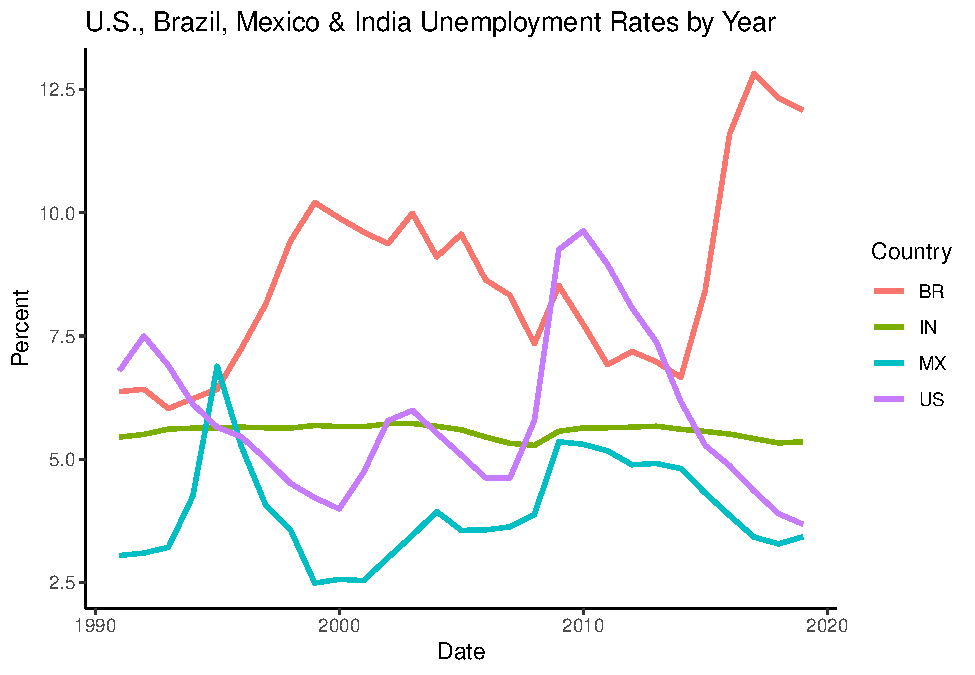
\includegraphics{econ200-book_files/figure-latex/unnamed-chunk-2-1.pdf}

\hypertarget{intro}{%
\chapter{Introduction}\label{intro}}

In Figure \ref{fig:unems} below, you will see the unemployment rate for four countries averaged over each year. The unemployment rate measures the percent of people who cannot find a job in the group of those people either working or looking for work. It seems like a mouthful, but we are estimating the proportion of people who are technically in the \emph{labor force}.

\begin{figure}

{\centering 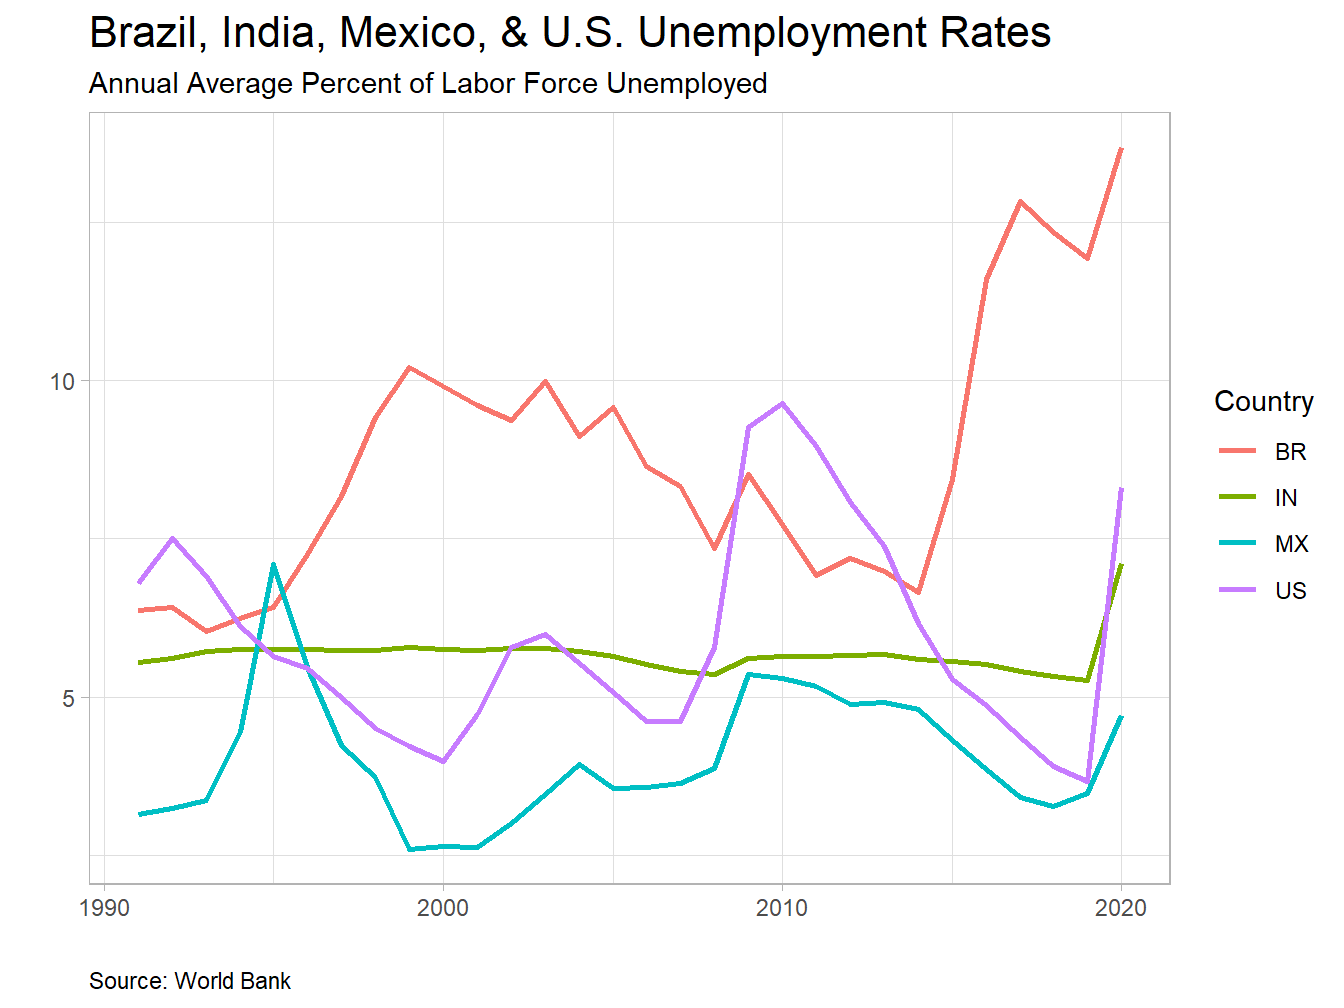
\includegraphics[width=0.8\linewidth]{econ200-book_files/figure-latex/unems-1} 

}

\caption{Unemployment Rates Around the World}\label{fig:unems}
\end{figure}

\begin{quote}
\textbf{Labor Force} is the sum of those who are employed and those actively looking for work.
\end{quote}

We measure the unemployment rate as:

\[ \text{Unemployment Rate} = \frac{\text{Unemployed}}{\text{Unemployed} + \text{Employed}} \times 100 \]

Something important about Figure \ref{fig:unems} is that we can see in some countries the unemployment rate is much higher than in other countries. Partially this is because we do not all use the same measurements for those who are either technically unemployed or working. However, if we assume countries do a consistent job in measuring these rates, the changes are still somewhat accurate. For example, in the United States a monthly survey of about 60,000 households counts those considered unemployed not just as those people collecting unemployment payments, but also includes all those people who have actively sought work in the past four weeks \href{https://www.bls.gov/cps/cps_htgm.htm}{(Bureau of Labor Statistics)}.

In recent months the COVID-19 crisis has gripped the world and put our global economy in a precarious position. As we can see from Figures \ref{fig:jobs} and \ref{fig:vmt} people who are newly jobless and travel in the U.S. have moved dramatically in opposite directions.

\begin{figure}

{\centering 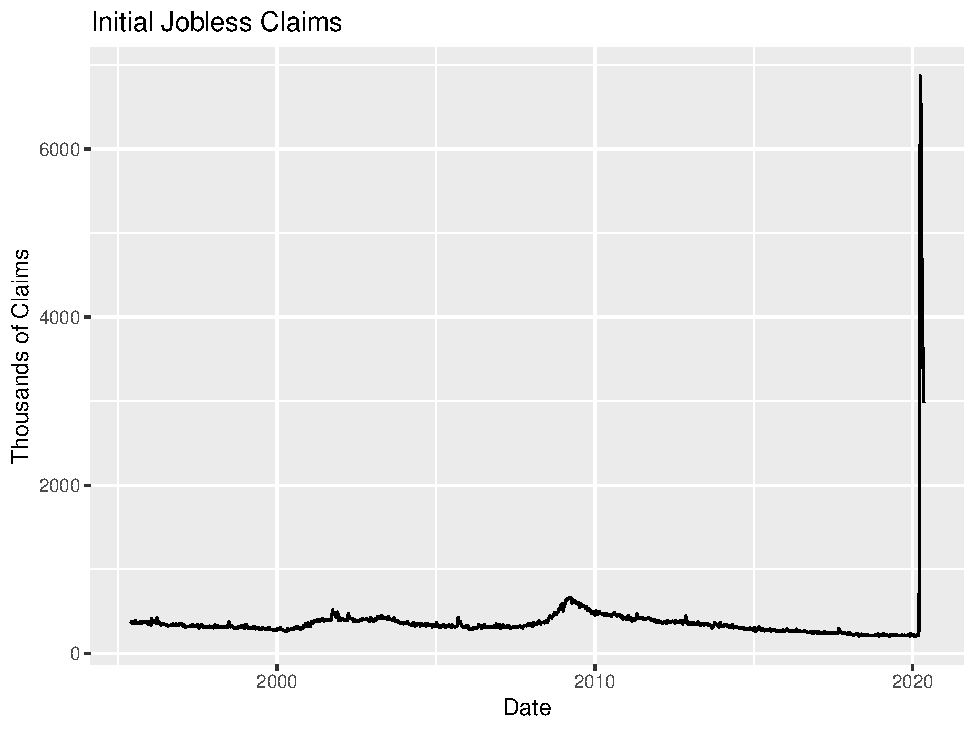
\includegraphics[width=0.8\linewidth]{econ200-book_files/figure-latex/jobs-1} 

}

\caption{Jobless Claims Skyrocket in 2020}\label{fig:jobs}
\end{figure}

\begin{figure}

{\centering 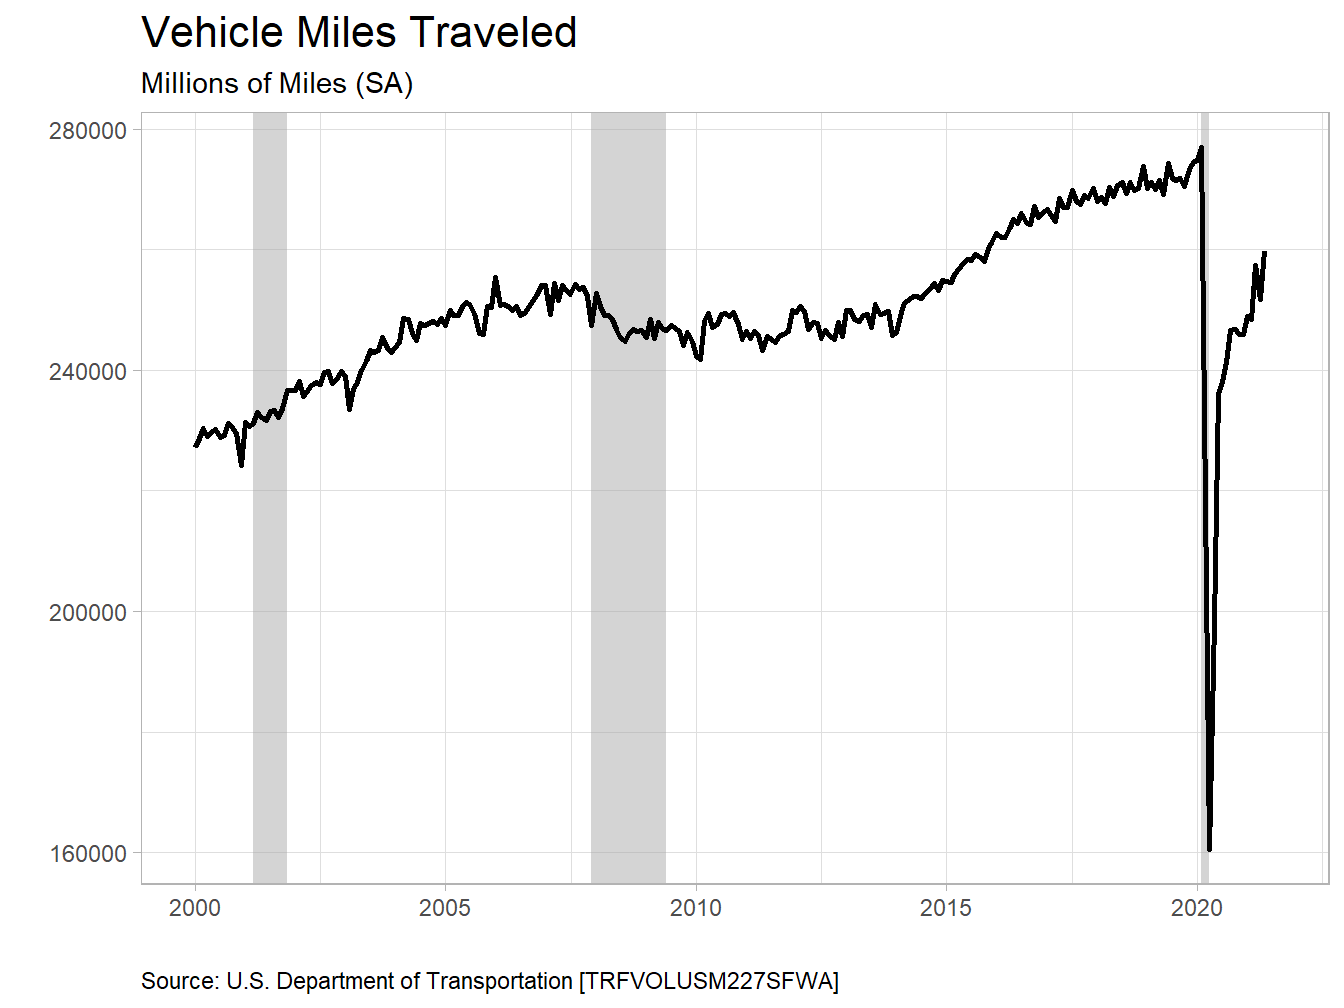
\includegraphics[width=0.8\linewidth]{econ200-book_files/figure-latex/vmt-1} 

}

\caption{Travel Collapses in 2020}\label{fig:vmt}
\end{figure}

Table \ref{tab:initial} shows the initial claims data for the past fifteen weeks, going back to the first weeks of the crisis in early March. Notice that the number of people filing for unemployment rose by a factor of more than ten! These unemployment claim numbers had literally never occurred in the U.S. before.

\begin{table}

\caption{\label{tab:initial}The Last 15 Weeks of Initial Unemployment Claims}
\centering
\begin{tabular}[t]{lr}
\toprule
Date & Claims\\
\midrule
2020-02-01 & 201000\\
2020-02-08 & 204000\\
2020-02-15 & 215000\\
2020-02-22 & 220000\\
2020-02-29 & 217000\\
\addlinespace
2020-03-07 & 211000\\
2020-03-14 & 282000\\
2020-03-21 & 3307000\\
2020-03-28 & 6867000\\
2020-04-04 & 6615000\\
\addlinespace
2020-04-11 & 5237000\\
2020-04-18 & 4442000\\
2020-04-25 & 3867000\\
2020-05-02 & 3176000\\
2020-05-09 & 2981000\\
\bottomrule
\end{tabular}
\end{table}

\hypertarget{literature}{%
\chapter{Literature}\label{literature}}

Here is a review of existing methods.

\hypertarget{methods}{%
\chapter{Methods}\label{methods}}

We describe our methods in this chapter.

\hypertarget{applications}{%
\chapter{Applications}\label{applications}}

Some \emph{significant} applications are demonstrated in this chapter.

\hypertarget{example-one}{%
\section{Example one}\label{example-one}}

\hypertarget{example-two}{%
\section{Example two}\label{example-two}}

\hypertarget{final-words}{%
\chapter{Final Words}\label{final-words}}

We have finished a nice book.

  \bibliography{refs.bib}

\end{document}
